\subsubsection{EXPRESS-based data models}\label{sec:express-based-data-models}



EXPRESS-based data models have data schemas specified in EXPRESS language \cite{iso2004express} and their data can be stored in STEP-File or STEP-XML formats.
EXPRESS is a standard data modeling language for product data that is defined in ISO 10303-11 \cite{iso2004express}, a part of ISO 10303 Product data representation and exchange standard, as known as ISO STEP (Standard for the Exchange of Product model data).
ISO STEP also specifies EXPRESS-G, a graphical notation for a subset of EXPRESS.
An EXPRESS-based data model may have more than one schemas, each of which address a specific subdomain of the domain.
These schemas may be related to each other via schema interfaces.
STEP-File (STEP Physical File, SPF, or STEP) \cite{iso2016stepfile} and STEP-XML \cite{iso2007stepxml} are two data serialization formats, accordingly defined in ISO 10303-21 and ISO 10303-28.


\textbf{Typical examples} of EXPRESS-based models are IFC (Industry Foundation Classes) and COBie (Construction Operations Building Information Exchange).

IFC is a platform neutral and open product data model, and is the most extensively utilized collaboration data format in BIM.
IFC is developed and published by buildingSMART as openBIM standard IFC (equivalent to ISO 13739:2013) \cite{iso2013ifc}.
Currently, two IFC specifications are officially in use: IFC2x3 TC1 \cite{liebich2007ifc2x3} and IFC4 Add2 \cite{liebich2016ifc4}, because the number of BIM software applications and software vendors granted with IFC4 certification is very little comparing with the ones with IFC2x3 certification.
Each IFC specification include the IFC Product data model (IFC Object model) in several languages: EXPRESS, EXPRESS-G, and XSD \cite{liebich2007ifc2x3, liebich2016ifc4}.
IFC-EXPRESS and IFC-XSD are \emph{almost} equivalent; their distinction is discussed in \autoref{sec:xsd-based-models}.
IFC datasets can be serialised in different file formats, namely IFC-SPF (IFC-STEP), IFC-XML (ifcXML), or IFC-ZIP (ifcZIP).
IFC-SPF datasets are based on STEP-file format and conform to IFC-EXPRESS schema.
Similarly, IFC-XML datasets are based on STEP-XML format and conform to IFC-XSD schema.
IFC-ZIP is a ZIP compressed format consisting of an embedded IFC-SPF.
In addition to the IFC Object model in formal languages, an IFC specification, i.e. an IFC Release documentation, also contain semantic explanations in informal languages, and IFC Property Set definitions (PSDD) in XSD (see details in \ref{sec:xsd-based-models}).


COBie is an international standard specification of information exchange to capture data during design, construction, and commissioning for handover to facility management \cite{bentley2013cobie, east2007construction}.
COBie, first was published by US Army Corps of Engineer in 2007 and today is jointly maintained by several buildingSMART organizations \cite{day2014problem, karlshoj2016delivering}.
COBie-compliant information can be delivered in four formats: COBie Spreadsheet XML, IFC-SPF, IFC-XML, and COBieLite RC 4 (XML).
COBie Spreadsheet XML, based on SpreadsheetML, is the most common format used by practitioners because it is editable with spreadsheet tools.
IFC-SPF and IFC-XML are used for the delivery of COBie data via IFC, consisting of two steps: (1) the exploration of the native model in IFC format, and (2) the transformation of the IFC model in COBie spreadsheet format \cite{karlshoj2016delivering}. 
As pointed out in \cite{yalcinkaya2015examining}, although "IFC is not all-in-one and the only source for the information requested in COBie specification", it "can be considered as the most convenient source for COBie extraction".
COBieLite is a new NIEM-conformant (National Information Exchange Model) XML format designed to support lightweight COBie information exchanges with Web Services.
Relationships between entities in this format are explicitly defined with XSD and it is free of unnecessary data about spreadsheets, text style and so on \cite{bogen2015cobielite}.
While COBieLite is still under development, the other three formats are officially approved in the British Standard BSI1192-4:2014 about making COBie mandatory for public commissions in UK from April 2016 \cite{karlshoj2016delivering}.



\begin{figure}
    \centering    
    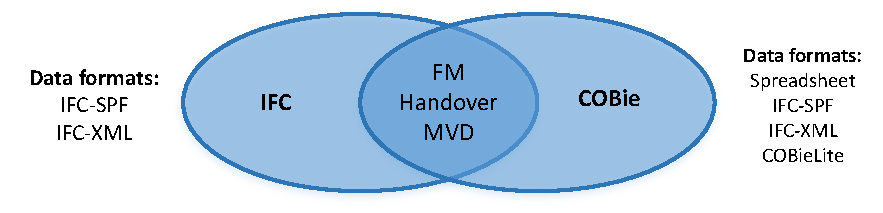
\includegraphics[width=\columnwidth]{images/ifc-and-cobie-2.pdf}
    \caption{Relation between IFC and COBie data}
    \label{fig:ifc-and-cobie}
\end{figure}






% All BIM tools, such as Revit, ArchiCAD or Tekla, besides their native data formats, must be able to produce and utilize one or more IFC data formats.






% As of now, IFC data schemas are the only EXPRESS-based data models used in BIM.
\textbf{An EXPRESS schema} consists of different kinds of declarations (see Listing \ref{lst:express-schema-declaration}).
% However, the import and constant declarations are currently unused in the IFC-EXPRESS data schemas.
However, as mentioned in \autoref{sec:scope-of-interest} functions (defined with keyword \texttt{FUNCTION}), procedures (\texttt{PROCEDURE}), global rules (\texttt{RULE}), local type rules (\texttt{WHERE}), and derived attributes (\texttt{DERIVE}) are out of consideration.



Therefore, only data type declarations \emph{without} constraints and derived attributes are needed for specifying the data structure in the physical data level.


% All declarations, except type declarations, are outside the range of consideration because:
% \begin{itemize}
% \item Only type declarations are used for describing
% % \emph{static}
% datasets in the physical data level, which are delivered in the STEP-File and STEP-XML formats.


% \item Declarations of functions (started with the keyword \texttt{FUNCTION}), procedures (\texttt{PROCEDURE}), rules (\texttt{RULE}), type constraints (\texttt{WHERE}), and derived attributes (\texttt{DERIVE}) contain executable statements and other programming operators, which cannot be represented in restricted OWL 2 profiles (see...).
% \item The IFC-EXPRESS data schemas are self-contained and do not import other schemas using declaration \texttt{REFERENCE FROM}.
% \item There is no declarations of constants (\texttt{CONSTANT}) in IFC-EXPRESS so far.
% \end{itemize}


\begin{lstlisting}[caption={The structure of an EXPRESS schema},label=lst:express-schema-declaration]
SCHEMA IFC4;

[import declarations]
[constant declarations]
[type declarations]
[function declarations]
[procedure declarations]
[rule declarations]

SCHEMA;
\end{lstlisting}




There are six groups of data types in EXPRESS:

\begin{itemize}

\item
\emph{Simple} data types are seven built-in types, including \texttt{STRING}, \texttt{INTEGER}, \texttt{REAL}, \texttt{NUMBER}, \texttt{BOOLEAN}, \texttt{LOGICAL}, and \texttt{BI\-NARY}.
The data type \texttt{NUMBER} is a super type of both \texttt{INTEGER} and \texttt{REAL}.
The data type \texttt{BOOLEAN} with two values \texttt{TRUE} and \texttt{FALSE} is traditionally used for Boolean logic.
Whereas, the data type \texttt{LOGICAL} with an additional value \texttt{UNKNOWN} is needed for different trivalent (three-valued) logics \cite{fronthofer2011manyvaluedlogics}.
% Truth values in trivalent logic may be represented numerically using various representations: (-1, 0, 1), (-1, 0, 0/1), (0, 1, 2) and so on.

\item
\emph{Entity} data types are almost similar to classes in traditional object-oriented programming (OOP) languages, with a few exceptions:
(i) they have no operations;
(ii) they contain derived attributes and type constraints, which are outside the range of consideration, as explained above;
(iii) they have inverse attributes, which are similar to inverse properties in OWL (see Section ...).
Like classes in Java and C{\#}, an entity data type has \emph{not more than one} super type.
However, attribute names of subtypes should not duplicate attribute names of their super types.
Nevertheless, there is no restrictions between attribute names in unrelated classes (it is important).
Each attribute has a certain data type, which can belong to any of the six data type groups.
In addition, the order of attribute declarations inside each entity data type is important because it is used for serialisation in the STEP-File format.

\item
\emph{Enumeration} data types represent fixed sets of possible string values. Different enumeration data types may have similar values.

\item
\emph{Select} data types are \emph{unions} of other data types.

\item
\emph{Aggregation} data types are \emph{unnamed} containers of values of exactly \emph{one} other data type
\footnote{In other data models, aggregation data usually consist of values from different types.}.
In other words, they are collection types in such languages like Java or C{\#}.
There are four types of aggregation: \texttt{ARRAY} (ordered, defined with start and end indexes), \texttt{LIST} (ordered, defined with minimum and maximum cardinalities), \texttt{SET} (unordered, all values are unique), and \texttt{BAG} (unordered, no duplicated values).
It is noteworthy that the aggregation type \texttt{BAG} is most likely never be used in practice.


\item
\emph{Defined} or \emph{named} data types are used as a simple way to \emph{name} and add constraints to another data type.
For instance, consider the sample defined types in Listing \ref{lst:express-defined-types}.
The type \texttt{Ifc\-Length\-Measure} is defined to assign a meaningful name to the simple type \texttt{REAL}.
The type \texttt{Ifc\-Positive\-Length\-Measure} is defined to restrict \texttt{Ifc\-Length\-Measure} to be positive and add a corresponding name.
The types \texttt{Ifc\-Complex\-Number} and \texttt{Ifc\-Compound\-Plane\-Angle\-Measure} are defined to identify unnamed aggregation types and also add some constraints.


% Each defined data type can be considered as a named subset (or an equivalent set) of another data type.
% Without going into detail of type constraints, we can say the following things about the defined data types in \ref{lst:express-defined-types}:
% \texttt{IfcPositiveLengthMeasure} \subseteq \texttt{IfcLengthMeasure} \equiv \texttt{REAL}


% Consider the sample types in Listing \ref{lst:express-defined-types}.
% The defined type \texttt{IfcPositiveLengthMeasure} is a subset of another defined type \texttt{IfcLengthMeasure}, which in turn is equal to the simple type \texttt{REAL}.
% The defined type \texttt{IfcBoxAlignment} is a subset of another defined type \texttt{IfcLabel}, which represents a subset \texttt{STRING}




\end{itemize}


\begin{lstlisting}[caption={Examples of defined data types},label=lst:express-defined-types]
TYPE IfcLengthMeasure = REAL;
END_TYPE;

TYPE IfcPositiveLengthMeasure = IfcLengthMeasure;
 WHERE
    WR1 : SELF > 0.;
END_TYPE;

TYPE IfcComplexNumber = ARRAY [1:2] OF REAL;
END_TYPE;

TYPE IfcCompoundPlaneAngleMeasure = LIST [3:4] OF INTEGER;
 WHERE
    MinutesInRange : ABS(SELF[2]) < 60;
    SecondsInRange : ABS(SELF[3]) < 60;
    MicrosecondsInRange : (SIZEOF(SELF) = 3) OR (ABS(SELF[4]) < 1000000);
    ...
END_TYPE;


\end{lstlisting}

% TYPE IfcBoxAlignment = IfcLabel;
%  WHERE
% 	WR1 : SELF IN ['top-left', 'top-middle', 'top-right', 'middle-left', 'center', 'middle-right', 'bottom-left', 'bottom-middle', 'bottom-right'];
% END_TYPE;

% TYPE IfcLabel = STRING(255);
% END_TYPE;



% According to the mapping methodology from IFC-EXPRESS to IFC-XSD, simple data types \texttt{STRING}, \texttt{INTEGER}, \texttt{REAL}, \texttt{NUMBER}, \texttt{BOOLEAN} are mapped to equivalent standard \texttt{XSD} types, namely \texttt{xs:string} (sometimes \texttt{xs:nor\-ma\-li\-zed\-String}), \texttt{xs:in\-te\-ger}, \texttt{xs:dou\-ble} (twice), and \texttt{xs:\-boo\-le\-an}.
% In the same time simple data types \texttt{LOGICAL} and \texttt{BINARY} are translated into user defined types \texttt{ifc:lo\-gi\-cal} and \texttt{ifc:hex\-Bi\-na\-ry}.


In the IFC-EXPRESS schema, all data types for calendar and duration values are defined types, not included in EXPRESS (Listing \ref{lst:express-calendar-types}).

\begin{lstlisting}[caption={Examples of calendar-related data types},label=lst:express-calendar-types]
TYPE IfcTime = STRING;
END_TYPE;

TYPE IfcTimeMeasure = REAL;
END_TYPE;

TYPE IfcTimeStamp = INTEGER;
END_TYPE;


TYPE IfcDate = STRING;
END_TYPE;

TYPE IfcDateTime = STRING;
END_TYPE;

TYPE IfcDuration = STRING;
END_TYPE;



\end{lstlisting}


TODO: Add some example of an entity data type


% <xs:simpleType name="IfcLogical">
% 		<xs:restriction base="ifc:logical"/>
% 	</xs:simpleType>
	
% 	<xs:simpleType name="IfcMassFlowRateMeasure">
% 		<xs:restriction base="xs:double"/>
% 	</xs:simpleType>
	
	
% 	<xs:simpleType name="IfcTime">
% 		<xs:restriction base="xs:normalizedString"/>
% 	</xs:simpleType>
% 	<xs:simpleType name="IfcTimeMeasure">
% 		<xs:restriction base="xs:double"/>
% 	</xs:simpleType>
% 	<xs:simpleType name="IfcTimeStamp">
% 		<xs:restriction base="xs:long"/>
% 	</xs:simpleType>
	
	
% 		<xs:simpleType name="IfcDate">
% 		<xs:restriction base="xs:normalizedString"/>
% 	</xs:simpleType>
% 	<xs:simpleType name="IfcDateTime">
% 		<xs:restriction base="xs:normalizedString"/>
% 	</xs:simpleType>











% EXPRESS defines 


% According to terminology of EXPRESS, 

% , which are a bit different to the data models used traditional OOP (object-oriented programming) languages.
% In particular, an attribute in EXPRESS may have multiple values, similarly to properties in OWL and unlike class attributes in traditional OOP.
% Another difference is that lists and sets in EXPRESS may have both minimum and maximum cardinalities, again similarly to OWL.
% ...
% Tabular and relational data models are related with such terms as tables, rows and columns.
% And for that reason, spreadsheets also belong to this category.



% \begin{table}[!th]
%     \centering
%     \begin{tabular}{c|c|c|c}
%         \hline
%         Group & EXPRESS-bases & XSD-based & Tabular \& relational data \\
%         \hline
%         Data schema & IFC-EXPRESS & IFC-XSD & \\
%         \hline
%     \end{tabular}
%     \caption{Caption}
%     \label{tab:my_label}
% \end{table}










% Firstly, 

% , such as 




% The SPF-based formats are the data formats 








% , which, however, have similar properties.
% They are: SPF, 




